\documentclass{beamer}

\usetheme{CambridgeUS}
%\usetheme{Luebeck}
\usecolortheme{beaver}
\useinnertheme{rectangles}
\usepackage[utf8]{inputenc}
\usepackage[czech]{babel}
\usepackage{graphicx}
\usepackage{amsmath}
\usepackage{color}
\usepackage{listings}
\lstset{
    breaklines=true,
    xleftmargin=\parindent,
    language=C++,
    showstringspaces=false,
    basicstyle=\footnotesize\ttfamily,
    keywordstyle=\color[rgb]{0,0,1},
    commentstyle=\color[rgb]{0.026,0.112,0.095},
    %identifierstyle=\color{blue},
    stringstyle=\color[rgb]{0.627,0.126,0.941},
}

\begin{document}
\setbeamertemplate{caption}{\raggedright\insertcaption\par}

\title[ReCodEx -- ReCodEx Code Examiner] % (optional, only for long titles)
{ReCodEx -- ReCodEx Code Examiner}
\author[Buchar, Polanka, Rozsíval, Stefan]{J. Buchar, M. Polanka, Š. Rozsíval, P. Stefan}
\institute[] % (optional)
{
  Matematicko-fyzikální fakulta\\
  Univerzita Karlova v Praze
}
\date[3. 12. 2016]{} % (optional)
\subject{Computer Science}
%\logo{
\includegraphics[width=0.2\textwidth]{images/logo_recodex.png}}
\titlegraphic{
\includegraphics[width=0.5\textwidth]{images/logo_recodex.png}}

\frame{\titlepage}

\section{ReCodEx}

\begin{frame}
	\frametitle{Osnova}
	\begin{itemize}
		\item Co je to ReCodEx?
		\item Praktická ukázka
		\item Architektura
		\begin{itemize}
			\item Komponenty
			\item Komunikace
		\end{itemize}
	\end{itemize}
\end{frame}

\begin{frame}
	\frametitle{Motivace}
	\begin{itemize}
		\item Zastaralý frontend CodExu
		\item Sandbox nepodporuje paralelní programy
		\item Omezená vyhodnocovací pipeline (kompilace/spuštění/vyhodnocení)
		\item Pevně svázané komponenty CodExu
	\end{itemize}
\end{frame}

\begin{frame}
	\frametitle{Praktická ukázka}
\end{frame}

\begin{frame}
	\frametitle{Architektura}
	\begin{itemize}
		\item Nezávislé komponenty, které spolu komunikují
		\item Backend zajišťuje vyhodnocování úloh
		\item REST API zpracovává a ukládá data
		\item Webová aplikace zpřístupňuje data uživatelům
	\end{itemize}
\end{frame}

\begin{frame}
	\frametitle{Komponenty a komunikace}
	\begin{center}
		\includegraphics[width=0.8\textwidth]{images/communication.png}
	\end{center}
\end{frame}

\begin{frame}
	\frametitle{Webová aplikace}
	\begin{itemize}
		\item ovládání systému uživateli
		\item SPA (single-page application)
		\item ECMAScript a HTML5
		\item knihovna React, framework Redux, \dots
		\item NodeJS server
	\end{itemize}
\end{frame}

\begin{frame}
	\frametitle{Webová aplikace II}
	\begin{center}
		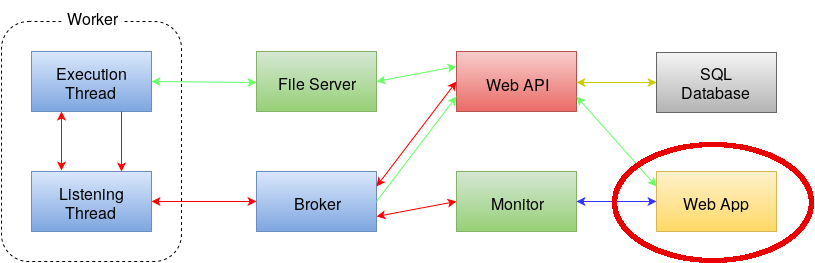
\includegraphics[width=0.8\textwidth]{images/communication-webapp.png}
	\end{center}
\end{frame}

\begin{frame}
	\frametitle{REST API}
	\begin{itemize}
		\item hlavní logika aplikace, ukládání dat
		\item PHP 7
		\item framework Nette, Doctrine, ZeroMQ nadstavba pro PHP, \dots
		\item Apache server s {\it mod\_php}
		\item MySQL databáze (MariaDB)
	\end{itemize}
\end{frame}

\begin{frame}
	\frametitle{REST API II}
	\begin{center}
		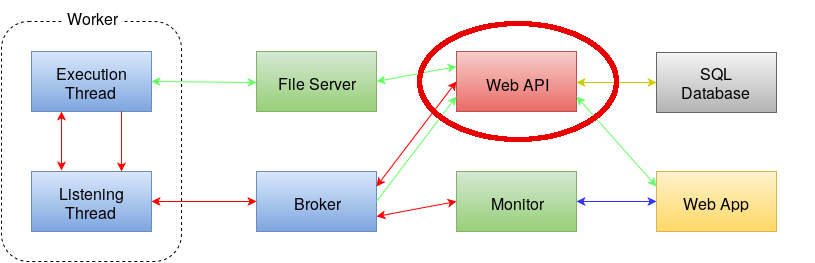
\includegraphics[width=0.8\textwidth]{images/communication-webapi.png}
	\end{center}
\end{frame}

\begin{frame}
	\frametitle{Broker}
	\begin{itemize}
		\item rozdělování práce mezi workery
		\item C++11
		\item ZeroMQ, libcurl, \dots
		\item \texttt{systemd} proces
	\end{itemize}
\end{frame}

\begin{frame}
	\frametitle{Broker II}
	\begin{center}
		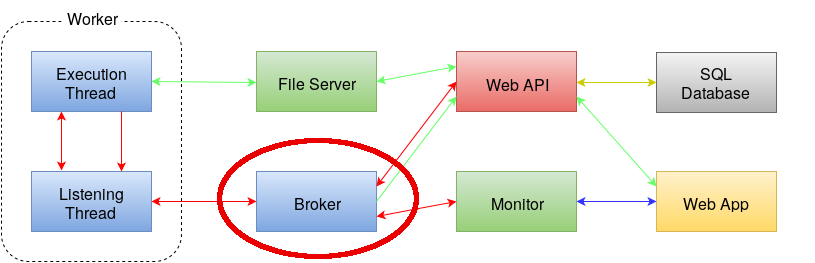
\includegraphics[width=0.8\textwidth]{images/communication-broker.png}
	\end{center}
\end{frame}

\begin{frame}
	\frametitle{Worker}
	\begin{itemize}
		\item bezpečné zpracování a vyhodnocení úlohy
		\item C++11
		\item ZeroMQ, libcurl, libarchive, \dots
		\item \texttt{systemd} proces
	\end{itemize}
\end{frame}

\begin{frame}
	\frametitle{Worker II}
	\begin{center}
		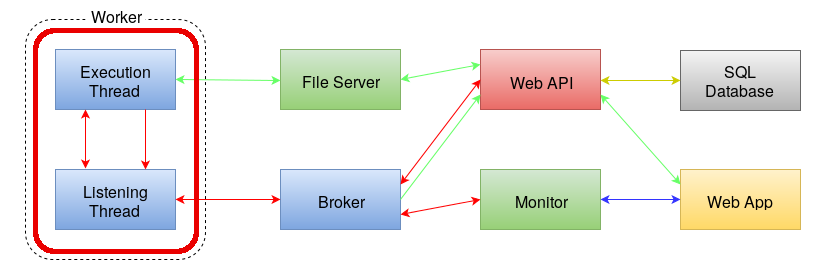
\includegraphics[width=0.8\textwidth]{images/communication-worker.png}
	\end{center}
\end{frame}

\begin{frame}
	\frametitle{Fileserver}
	\begin{itemize}
		\item skladování pomocných souborů k úlohám a studentských řešení
		\item Python 3
		\item Flask, \dots
		\item uWSGI aplikace
	\end{itemize}
\end{frame}

\begin{frame}
	\frametitle{Fileserver II}
	\begin{center}
		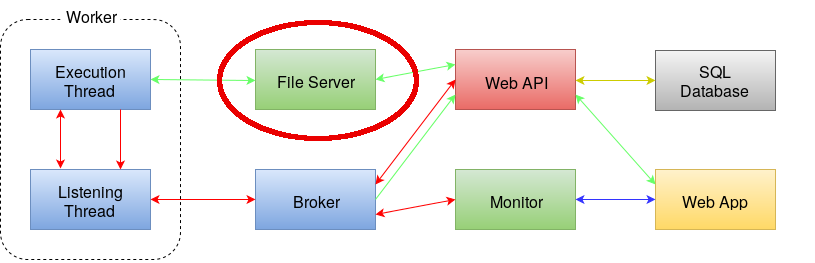
\includegraphics[width=0.8\textwidth]{images/communication-fileserver.png}
	\end{center}
\end{frame}

\begin{frame}
	\frametitle{Monitor}
	\begin{itemize}
		\item hlášení postupu vyhodnocení uživatelům
		\item Python 3
		\item ZeroMQ nadstavba pro Python, websockets, asyncio, \dots
		\item \texttt{systemd} proces
	\end{itemize}
\end{frame}

\begin{frame}
	\frametitle{Monitor II}
	\begin{center}
		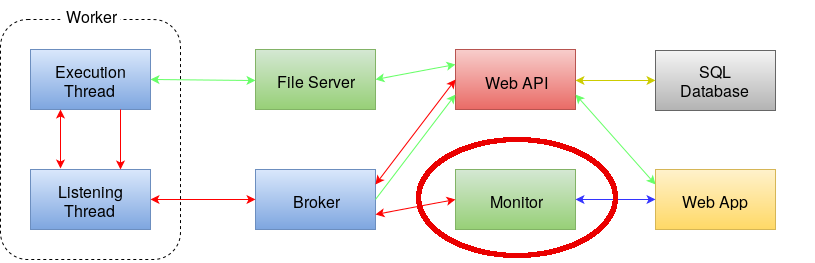
\includegraphics[width=0.8\textwidth]{images/communication-monitor.png}
	\end{center}
\end{frame}

\begin{frame}
	\frametitle{Hodnocení}
	\begin{itemize}
		\item návrh a implementace nového vyhodnocovacího systému
		\item zapracování požadavků MFF UK
		\item moderní technologie, rozšiřitelnost, bezpečnost
		\item testování
		\item plné nasazení v příštím akademickém roce
	\end{itemize}
\end{frame}

\section{Závěr}
\begin{frame}
	\frametitle{Závěr}
	\centering
	Děkujeme za pozornost.\\
	\LARGE{Otázky?}
\end{frame}

\end{document}
